% EOS 513 REPORT
\documentclass[jgrga]{agutex}
\usepackage{graphicx}
\usepackage{amsmath}
\usepackage{color}

\newcommand{\bt}[1]{\textbf{#1}}
\newcommand{\bc}[1]{\mathcal{\textbf{#1}}}
\newcommand{\ub}[1]{\underbrace{#1}}
\newcommand{\ob}[1]{\overbrace{#1}}
%%%%%%%%%%%%%%%%%%%%%%%%%%%%%%%%%%%%%%%%%%%%%%%%%%%%%%%%%%%%%%%%%%%%%%%%%
% OPTIONAL:
% To produce a two-columned version:
% \documentclass[jgrga]{AGUTeX}

% Two-columned format can be used to estimate the number of pages
% for the final published PDF.

% PLEASE USE THE DRAFT OPTION TO SUBMIT YOUR PAPERS.
%%%%%%%%%%%%%%%%%%%%%%%%%%%%%%%%%%%%%%%%%%%%%%%%%%%%%%%%%%%%%%%%%%%%%%%%%
% OPTIONAL:
% To create numbered lines:

% If you don't already have lineno.sty, you can download it from
% http://www.ctan.org/tex-archive/macros/latex/contrib/ednotes/
% (or search the internet for lineno.sty ctan), available at TeX Archive Network (CTAN).
% Take care that you always use the latest version.

% To activate the commands, uncomment \usepackage{lineno}
% and \linenumbers*[1]command, below:

% \usepackage{lineno}
% \linenumbers*[1]

%  To add line numbers to lines with equations:

%  \begin{linenomath*}
%  \begin{equation}
%  \end{equation}
%  \end{linenomath*}
%%%%%%%%%%%%%%%%%%%%%%%%%%%%%%%%%%%%%%%%%%%%%%%%%%%%%%%%%%%%%%%%%%%%%%%%%
% Figures and Tables
%
% When submitting articles through the GEMS system:
% COMMENT OUT ANY COMMANDS THAT INCLUDE GRAPHICS.
% (See FIGURES section near the end of the file.)
%
% DO NOT USE \psfrag or \subfigure commands.
%
%  Figures and tables should be placed AT THE END OF THE ARTICLE,
%  after the references.
%
%  Uncomment the following command to include .eps files
%  (comment out this line for draft format):
% \usepackage[dvips]{graphicx}
%
%  Uncomment the following command to allow illustrations to print
%   when using Draft:
%  \setkeys{Gin}{draft=false}
%
% Substitute one of the following for [dvips] above
% if you are using a different driver program and want to
% proof your illustrations on your machine:
%
% [xdvi], [dvipdf], [dvipsone], [dviwindo], [emtex], [dviwin],
% [pctexps],  [pctexwin],  [pctexhp],  [pctex32], [truetex], [tcidvi],
% [oztex], [textures]
%
% See how to enter figures and tables at the end of the article, after
% references.
%
%% ------------------------------------------------------------------------ %%
%
%  ENTER PREAMBLE
%
%% ------------------------------------------------------------------------ %%

% Author names in capital letters:
\authorrunninghead{MATHARU GIAN, BEN POSTLETHWAITE}

% Shorter version of title entered in capital letters:
\titlerunninghead{DECONVOLUTION L2 / L1 COMPARISON}

% Author mailing address: please repeat this command for
% each author and alphabetize authors:

%\authoraddr{R. C. Bales,
%Department of Hydrology and Water Resources, University of
%Arizona, Harshbarger Building 11, Tucson, AZ 85721, USA.
%(roger@hwr.arizona.edu)}

%\authoraddr{J. R. McConnell, Division of Hydrologic
%Sciences, 123 Main Street, Desert Research Institute, Reno, NV
%89512, USA.}

%\authoraddr{E. Mosley-Thompson, Department of Geography,
%Ohio State University, 123 Orange Boulevard, Columbus, OH 43210,
%USA.}

%\authoraddr{R. Williams, Department of Space Sciences, University of
%Michigan, 123 Brown Avenue, Ann Arbor, MI 48109, USA.}

%\authoraddr{Francesco Visconti, Dipartimento di Idraulica,
%Trasporti ed Infrastrutture Civili, Politecnico di Torino,
%Corso Duca degli Abruzzi 24, I-10129, Torino, Italy.

\begin{document}

%% ------------------------------------------------------------------------ %%
%
%  TITLE
%
%% ------------------------------------------------------------------------ %%


\title{Sparsity Promoting L1 Deconvolution: Application for a Global Seismology Parameter Search}
%
% e.g., \title{Terrestrial ring current:
% Origin, formation, and decay $\alpha\beta\Gamma\Delta$}
%

%% ------------------------------------------------------------------------ %%
%
%  AUTHORS AND AFFILIATIONS
%
%% ------------------------------------------------------------------------ %%


%Use \author{\altaffilmark{}} and \altaffiltext{}

% \altaffilmark will produce footnote;
% matching \altaffiltext will appear at bottom of page.

% \authors{R. C. Bales,\altaffilmark{1}
% E. Mosley-Thompson,\altaffilmark{2} R. Williams,\altaffilmark{3}
% J. R. McConnell\altaffilmark{4}, and Francesco Visconti\altaffilmark{5}}

%\altaffiltext{1}{Department of Hydrology and Water Resources,
%University of Arizona, Tucson, Arizona, USA.}

%\altaffiltext{2}{Department of Geography, Ohio State University,
%Columbus, Ohio, USA.}

%\altaffiltext{3}{Department of Space Sciences, University of
%Michigan, Ann Arbor, Michigan, USA.}

%\altaffiltext{4}{Division of Hydrologic Sciences, Desert Research
%Institute, Reno, Nevada, USA.}

%\altaffiltext{5}{Dipartimento di Idraulica, Trasporti ed
%Infrastrutture Civili, Politecnico di Torino, Turin, Italy.}

%% ------------------------------------------------------------------------ %%
%
%  ABSTRACT
%
%% ------------------------------------------------------------------------ %%

% >> Do NOT include any \begin...\end commands within
% >> the body of the abstract.

\begin{abstract}
This report will outline an attempt to utilize the inherent sparsity in seismic receiver functions in order to provide better deconvolution results than the often utilized damped-L2 methods. By promoting sparsity with the wavelet transform the use of sparse solvers such as SPGL1 becomes possible. Synthetic tests are performed using the damped L2 convolution as well as the sparse wavelet transform L1 minimization using several wavelet basis. Real data is employed and the deconvolved results from the competing methods are used for an actual parameter grid search. The final results of the grid search are then compared. Further work on the sparse-in-wavelets L1 algorthim will be required if it is to beat the damped-L2 algorthim currently being employed.
\end{abstract}

%% ------------------------------------------------------------------------ %%
%
%  BEGIN ARTICLE
%
%% ------------------------------------------------------------------------ %%

% The body of the article must start with a \begin{article} command
%
% \end{article} must follow the references section, before the figures
%  and tables.

\begin{article}

%% ------------------------------------------------------------------------ %%
%
%  TEXT
%
%% ------------------------------------------------------------------------ %%

\section{Introduction}

Extracting material properties from seismic data spans industry and the research community. In the global seismic community material properties of the crust have been sought to validate existing geological models or provide clues for new ones. A good example of this is Poisson's ratio, which is the ratio between compression along one axis to extension on another when a material is stretched (see figure 1). Poisson's ratio is given by:
\[ \sigma = \frac{1}{2} \frac{ \left( \frac{ V_p }{ V_s } \right)^2 - 2 }{ \left( \frac{ V_p }{ V_s } \right)^2 - 1 } \]

\begin{figure}
\noindent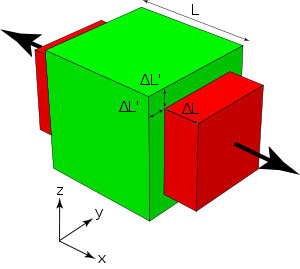
\includegraphics[width=18pc]{PoissonRatio.png}
\caption{Poissons Ratio is the ratio of compression along one axis to extension along another}
\end{figure}

where the seismic velocities $V_p$ and $V_s$ determine the property entirely. Because of the direct link between seismic properties and Poisson's ratio this material property has been sought in numerous seismic studies such as Kanamori (2000) and Snyder (2010). All of these studies have performed a parameter search for $R = \frac{V_p}{V_s}$ and provided a background estimate for $V_p$. This allows for fast computation through a grid search and avoids the problem of the low-dependency of $V_p$ in the grid search equations. Although Poisson's ratio can be estimated from $R$ better geological constraints would be possible if $V_p$ and $V_s$ were resolved uniquely. 

\section{The Problem}

In order to differentiate between $V_p$ and $V_s$ the travel times from seperate arrivals of energy must be compared. The first arrival a seismic station will pick up after the onset of an earthquake is from the higher velocity P-wave. The impulsive character and high amplitude of the P-wave arrival allow it to be windowed and filtered and used as an approximation for the source. There are three more arrivals of interest. The Ps arrival, which is P-energy converted to S-wave energy at the Moho boundary between the crust and the mantle. Two further arrivals follow which are the reflections from the free surface which have reflected again off the Moho and recorded at the station, figure (2). These reflected arrivals are usually of lower amplitude and often less well defined in the seismogram. If the three S-wave arrivals - the Ps, PpPs and PsPs - can be located in time this provides the data in which a model may be fit. Owing to the fact that the S-wave phases all travel within the same crustal thickess $H$, dividing the S-wave relected phases by the initial Ps phase will remove the dependence on crustal thickness. The traveltime ratios are then dependent on $V_p$ and $V_s$ only (Bostock, 2010). With this information a 2D grid search over the travel time equations with respect to $V_p$ and $V_s$ can be performed. The parameter $V_p$ is not very sensitive to the traveltime differences between the S-wave phases, thus a very impulsive deconvolution result is needed to steepen the gradient in $V_p$ space. 


\begin{figure}
\noindent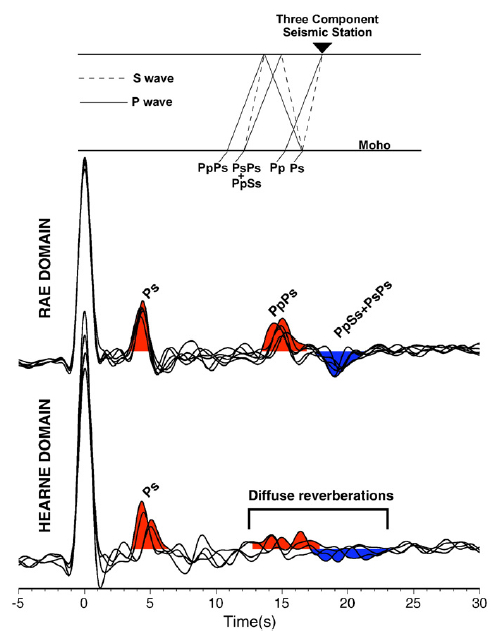
\includegraphics[width=18pc]{reflectRecs.jpg}
\caption{Top: Shows direct phases Pp and Ps from a seismic event hitting receiver. Also the reflected phases PpPs and PsPs are shown. The phases ending with 's' are the phases hitting the station as S-waves. These S-wave phases are used as the primary data, the direct Pp phase is used as the source, and the two are deconvolved to attain the receiver functions shown at Bottom: The receiver functions attained from deconvolution. Depending on the quality of the data and the sharpness of the deconvolution, the results may look like those given for the Rae Domain -better- or the Hearne Domain -worse.}
\end{figure}


\section{Deconvolution - L2}
Currently simultaneous deconvolution with generalized cross validation is being employed as it performs well and is very fast. Since division in the fourier basis is deconvolution in time we can write:
\[ \bc{R} = \bc{F}^{-1}[\bc{G}(\omega)]  \]
where
\[ \bc{G}(\omega) = \left[ \frac{\sum_n^N \bt{S}_n\bt{P}_n^*}{\sum_n^N \bt{P}_n\bt{P}_n^* + \delta}  \right] \].
Here $\bc{F}$ is the Fourier transform, $\bc{G}$ is the model, $\bt{S}$ is a matrix of S-wave seismograms, $\bt{P}$ is a matrix of P-wave source coda, $*$ is the complex conjugate and $\delta$ is the regularization parameter. $\delta$ is chosen by minimizing the Generalized Cross Validation function with respect to $\delta$:
\[ \text{min} \left( \frac{ \sum_n^N \sum_m^M 
 \left( \ob{ \bt{S}_n(\omega_m) - \bt{P}(\omega_m) \left[ \frac{\sum_n^N \bt{S}_n\bt{P}_n^*} {\sum_n^N \bt{P}_n\bt{P}_n^* + \delta}  \right]}^{\text{\textcolor{red}{ Misfit: more accurate with $\delta\rightarrow0$. Less Stable }}} \right)^2}  { \left( 
\ub{  NM - \sum_m^M  \frac {\sum_n^N \bt{P}_n\bt{P}_n^*}  {\sum_n^N \bt{P}_n\bt{P}_n^* + \delta}  }_{\text{\textcolor{red}{ {As $\delta$ increases denominator increases, promotes stability.}}}} \right)^2  }  \right)  \] 

Since the sharpness of the deconvolution helps determine the confidence level contours on the final parameter estimation the prospect of a better deconvolution methods is very appealing. As the earth model being used in this parameter search is a simple layered model and the data is piecewise smooth the wavelet transform could be effectively used to promote sparsity. If we could leverage this fact and use an L1 technique which promotes sparse solutions we may be able to increase the accuracy of the deconvolved receiver functions. 


\section{Future Work}
Even with a fairly preliminary L1 minimization setup the results are encouraging. Further work could focus on the 2D receiver function plots and usage of curvelets to interpolate between poor data. This would significantly improve the estimates made by the grid search. While redundant wavelet dictionaries were employed in the non-spline cases these authors are currently unsure if the B-spline methods were shift-invariant or not. This will require further investigation. Also during a recent presentation of the work contained in this report Felix Herrmann suggested looking at Radon Transformations. Both authors are unsure of the utility of these transformations and this will also require further research. However, with a sophisticated tool-chain in place we believe that L1 minimization and the utilization of sparsity inherent in this problem will result in better deconvolution than the current L2 method being employed. Since there is a large body of global seismological work which has been built on results from L2 deconvolution there is a lot of potential to apply these methods to other problems. Along the same lines, once sparsity is being utilized, the larger compressive sensing framework should surely find a place in the global seismic research community. There is vast potential in this arena and likely many exciting avenues for phd research. Both the authors of this report are interested in exploring this new paradigm further in the context of global seismology.

%Deconvolution is a common yet difficult step in processing and analysis in many fields of science and technology. In the field of seismology deconvolution arises more often than most and due to the structural complexity and ambiguity of the earth poses a particularly challenging problem.

%%% End of body of article:

%%%%%%%%%%%%%%%%%%%%%%%%%%%%%%%%
%% Optional Appendix goes here
%
% \appendix resets counters and redefines section heads
% but doesn't print anything.
% After typing  \appendix
%
% \section{Here Is Appendix Title}
% will show
% Appendix A: Here Is Appendix Title
%
%%%%%%%%%%%%%%%%%%%%%%%%%%%%%%%%%%%%%%%%%%%%%%%%%%%%%%%%%%%%%%%%
%
% Optional Glossary or Notation section, goes here
%
%%%%%%%%%%%%%%
% Glossary is only allowed in Reviews of Geophysics
% \section*{Glossary}
% \paragraph{Term}
% Term Definition here
%
%%%%%%%%%%%%%%
% Notation -- End each entry with a period.
% \begin{notation}
% Term & definition.\\
% Second term & second definition.\\
% \end{notation}
%%%%%%%%%%%%%%%%%%%%%%%%%%%%%%%%%%%%%%%%%%%%%%%%%%%%%%%%%%%%%%%%
%
%  ACKNOWLEDGMENTS

\begin{acknowledgments}
(Text here)
\end{acknowledgments}

%% ------------------------------------------------------------------------ %%
%%  REFERENCE LIST AND TEXT CITATIONS
%
% Either type in your references using
% \begin{thebibliography}{}
% \bibitem{}
% Text
% \end{thebibliography}
%
% Or,
%
% If you use BiBTeX for your references, please produce your .bbl
% file and copy the contents into your paper here.
%
% Follow these steps:
% 1. Run LaTeX on your LaTeX file.
%
% 2. Run BiBTeX on your LaTeX file.
%
% 3. Open the new .bbl file containing the reference list and
%   copy all the contents into your LaTeX file here.
%
% 4. Comment out the old \bibliographystyle and \bibliography commands.
%
% 5. Run LaTeX on your new file before submitting.
%
% AGU DOES NOT WANT a .bib or a .bbl file. Please copy in the contents of your .bbl file here.

\begin{thebibliography}{}

\bibitem[{\textit{Herrmann}(2012)}]{herrmann}
Herrmann, F. J., (2012), Class material from EOS 513: Imaging and Estimation with Wavelets, {\it University of British Columbia}

\bibitem[{\textit{Bostock}(2010)}]{bostock}
Bostock, M. G., Kumar, M. R., (2010), Bias in seismic estimates of crustal properties, {\it Geophysical Journal International,} \textit{182}, 403--407.

\bibitem[{\textit{Thompson et al}(2010)}]{thompson}
Thompson, D. A., Bastow, I.D., Helffrich, G., Kendall, J-M., Wookey, J., Snyder, D.B., Eaton, D.W., (2010), Precambrian crustal evolution: Seismic constraints from the Canadian Shield, {\it Earth and Planetary Science Letters,} \textit{297}, 655--666.

\bibitem[{\textit{Kanamori et al.}(2000)}]{kanamori}
Kanamori, H. (2000), Moho depth variation in southern California from teleseismic receiver functions, {\it Geophysical Research,} \textit{105}, 2969--2980.

%\bibitem[{\textit{Kilby et al.}(2008)}]{jskilbye}
%Kilby, J. S., S. Smith, and R. Jones (2008), Invention of the
%integrated circuit, {\it IEEE Trans. Electron Devices,} \textit{23},
%648--650.

\end{thebibliography}

%Reference citation examples:

%...as shown by \textit{Kilby} [2008].
%...as shown by {\textit  {Lewin}} [1976], {\textit  {Carson}} [1986], {\textit  {Bartholdy and Billi}} [2002], and {\textit  {Rinaldi}} [2003].
%...has been shown [\textit{Kilby et al.}, 2008].
%...has been shown [{\textit  {Lewin}}, 1976; {\textit  {Carson}}, 1986; {\textit  {Bartholdy and Billi}}, 2002; {\textit  {Rinaldi}}, 2003].


%...as shown by \citet{jskilby}.
%...as shown by \citet{lewin76}, \citet{carson86}, \citet{bartoldy02}, and \citet{rinaldi03}.
%...has been shown \citep{jskilbye}.
%...has been shown \citep{lewin76,carson86,bartoldy02,rinaldi03}.
%
% Please use ONLY \citet and \citep for reference citations.
% DO NOT use other cite commands (e.g., \cite, \citeyear, \nocite, \citealp, etc.).

%% ------------------------------------------------------------------------ %%
%
%  END ARTICLE
%
%% ------------------------------------------------------------------------ %%

\end{article}

%% Enter Figures and Tables here:
%\begin{figure*}
%\noindent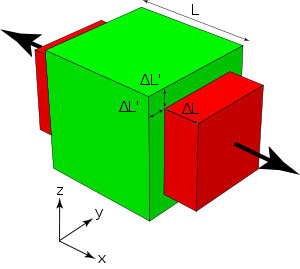
\includegraphics[width=10pc]{PoissonRatio.png}
%\caption{Poissons Ratio is the ratio of compression along one axis to extension along another}
%\end{figure*}

% When submitting articles through the GEMS system:
% COMMENT OUT ANY COMMANDS THAT INCLUDE GRAPHICS.
%
% FOR FIGURES, DO NOT USE \psfrag or \subfigure commands.
%
% Figure captions go below the figure.
% Table titles go above tables; all other caption information
%  should be placed in footnotes below the table.


\end{document}

% DRAFT figure/table, including eps graphics
%
% \begin{figure}
% \noindent\includegraphics[width=20pc]{samplefigure.eps}
% \caption{Caption text here}
% \end{figure}
% \end{document}
%
% \begin{table}
% \caption{}
% \end{table}
%
% ---------------
% TWO-COLUMN figure/table
%
% \begin{figure*}
% \noindent\includegraphics[width=39pc]{samplefigure.eps}
% \caption{Caption text here}
% \end{figure*}
%
% \begin{table*}
% \caption{Caption text here}
% \end{table*}
%
% ---------------
% EXAMPLE TABLE
%
%\begin{table}
%\caption{Time of the Transition Between Phase 1 and Phase 2\tablenotemark{a}}
%\centering
%\begin{tabular}{l c}
%\hline
% Run  & Time (min)  \\
%\hline
%  $l1$  & 260   \\
%  $l2$  & 300   \\
%  $l3$  & 340   \\
%  $h1$  & 270   \\
%  $h2$  & 250   \\
%  $h3$  & 380   \\
%  $r1$  & 370   \\
%  $r2$  & 390   \\
%\hline
%\end{tabular}
%\tablenotetext{a}{Footnote text here.}
%\end{table}

% See below for how to make landscape/sideways figures or tables.

\end{document}

%%%%%%%%%%%%%%%%%%%%%%%%%%%%%%%%%%%%%%%%%%%%%%%%%%%%%%%%%%%%%%%

%More Information and Advice:

%% ------------------------------------------------------------------------ %%
%
%  SECTION HEADS
%
%% ------------------------------------------------------------------------ %%

% Capitalize the first letter of each word (except for
% prepositions, conjunctions, and articles that are
% three or fewer letters).

% AGU follows standard outline style; therefore, there cannot be a section 1 without
% a section 2, or a section 2.3.1 without a section 2.3.2.
% Please make sure your section numbers are balanced.
% ---------------
% Level 1 head
%
% Use the \section{} command to identify level 1 heads;
% type the appropriate head wording between the curly
% brackets, as shown below.
%
%An example:
%\section{Level 1 Head: Introduction}
%
% ---------------
% Level 2 head
%
% Use the \subsection{} command to identify level 2 heads.
%An example:
%\subsection{Level 2 Head}
%
% ---------------
% Level 3 head
%
% Use the \subsubsection{} command to identify level 3 heads
%An example:
%\subsubsection{Level 3 Head}
%
%---------------
% Level 4 head
%
% Use the \subsubsubsection{} command to identify level 3 heads
% An example:
%\subsubsubsection{Level 4 Head} An example.
%
%% ------------------------------------------------------------------------ %%
%
%  IN-TEXT LISTS
%
%% ------------------------------------------------------------------------ %%
%
% Do not use bulleted lists; enumerated lists are okay.
% \begin{enumerate}
% \item
% \item
% \item
% \end{enumerate}
%
%% ------------------------------------------------------------------------ %%
%
%  EQUATIONS
%
%% ------------------------------------------------------------------------ %%

% Single-line equations are centered.
% Equation arrays will appear left-aligned.

%Math coded inside display math mode \[ ...\]
% will not be numbered, e.g.,:
% \[ x^2=y^2 + z^2\]

% Math coded inside \begin{equation} and \end{equation} will
% be automatically numbered, e.g.,:
% \begin{equation}
% x^2=y^2 + z^2
% \end{equation}

% IF YOU HAVE MULTI-LINE EQUATIONS, PLEASE
% BREAK THE EQUATIONS INTO TWO OR MORE LINES
% OF SINGLE COLUMN WIDTH (20 pc, 8.3 cm)
% using double backslashes (\\).

% To create multiline equations, use the
% \begin{eqnarray} and \end{eqnarray} environment
% as demonstrated below.
%\begin{eqnarray}
%  x_{1} & = & (x - x_{0}) \cos \Theta \nonumber \\
%        && + (y - y_{0}) \sin \Theta  \nonumber \\
%  y_{1} & = & -(x - x_{0}) \sin \Theta \nonumber \\
%        && + (y - y_{0}) \cos \Theta.
%\end{eqnarray}

%If you don't want an equation number, use the star form:
%\begin{eqnarray*}...\end{eqnarray*}

% Break each line at a sign of operation
% (+, -, etc.) if possible, with the sign of operation
% on the new line.

% Indent second and subsequent lines to align with
% the first character following the equal sign on the
% first line.

% Use an \hspace{} command to insert horizontal space
% into your equation if necessary. Place an appropriate
% unit of measure between the curly braces, e.g.
% \hspace{1in}; you may have to experiment to achieve
% the correct amount of space.


%% ------------------------------------------------------------------------ %%
%
%  EQUATION NUMBERING: COUNTER
%
%% ------------------------------------------------------------------------ %%

% You may change equation numbering by resetting
% the equation counter or by explicitly numbering
% an equation.

% To explicitly number an equation, type \eqnum{}
% (with the desired number between the brackets)
% after the \begin{equation} or \begin{eqnarray}
% command.  The \eqnum{} command will affect only
% the equation it appears with; LaTeX will number
% any equations appearing later in the manuscript
% according to the equation counter.
%

% If you have a multiline equation that needs only
% one equation number, use a \nonumber command in
% front of the double backslashes (\\) as shown in
% the multiline equation above.

%% ------------------------------------------------------------------------ %%
%
%  LANDSCAPE/SIDEWAYS FIGURE AND TABLE EXAMPLES
%
%% ------------------------------------------------------------------------ %%
%
% For figures, add \usepackage{lscape} to the file and the landscape.sty style file
% to the paper folder.
%
% \begin{figure*}[p]
% \begin{landscapefigure*}
% Illustration here.
% \caption{caption here}
% \end{landscapefigure*}
% \end{figure*}
%
% For tables, add \usepackage{rotating} to the paper and add the rotating.sty file to the folder.
%
% AGU prefers the use of {sidewaystable} over {landscapetable} as it causes fewer problems.
%
% \begin{sidewaystable}
% \caption{}
% \begin{tabular}
% Table layout here.
% \end{tabular}
% \end{sidewaystable}
%
%

